%!TEX root = ../summaries.tex

\chapter{Learning from humans}

\section{Imitation Learning, Part 1}

\url{https://youtu.be/kGc8jOy5_zY}

\begin{itemize}
    \item Differences when moving from prediction to control for AI systems
    \begin{itemize}
        \item No longer i.i.d.
        \item From ground truth supervision to high-level, abstract goal.
        \item Objective: from predict label to accomplish task.
        \item In real world, some prediction systems also have feedback issues: e.g.\@ traffic prediction system used and affects traffic.
    \end{itemize}
    \item Terminology.
    \begin{itemize}
        \item $\bf o_t$: observation.
        \item $\bf a_t$: action.
        \item $\bf s_t$: state (underlying variables in model).
        \item $\pi_\theta(\bf a_t \mid \bf o_t)$ or $\pi_\theta(\bf a_t \mid \bf s_t)$: policy.
        \item When policy depends on state, it is \emph{fully observed}.
        \begin{figure}[h!]
            \centering
            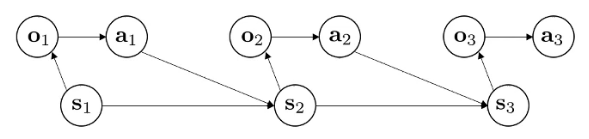
\includegraphics[width=.95\linewidth]{images/state-bayes-net.png}
            \caption{Bayes' net for the states, observations and actions}
            \label{fig:bayes net states}
        \end{figure}
    \end{itemize}
    \item Initiation learning: supervised learning.
    \begin{itemize}
        \item \emph{Behaviour cloning}.
        \item Doesn't work in theory: small mistakes compound, and we quickly diverge from training distribution.
        \item Works reasonably well in practice, given enough training data.
    \end{itemize}
\end{itemize}


\section{Learning from Human Preferences}

\url{https://openai.com/blog/deep-reinforcement-learning-from-human-preferences/}

\begin{itemize}
    \item Using feedback to infer goal.
    \item Builds model of goal based on feedback.
    \item Learns also when to ask for feedback.
    \item Trained on various games.
    \item Sometimes does better using human feedback than game's actual reward function (the score), since human shapes the reward function better.
    \item Limited by human evaluators intuition on what looks correct.
    \begin{itemize}
        \item On one task, learned to trick human using optical illusion.
    \end{itemize}
\end{itemize}